\documentclass[12pt,a4paper]{article}
\usepackage{times}
\usepackage{durhampaper}
\usepackage{harvard}
\usepackage{url}
\usepackage{graphicx}
\citationmode{abbr}
\bibliographystyle{agsm}

\title{Cloud-based RAW image editing}
\author{Ryan Collins}
\supervisor{Dr Tom Friedetzky}
\student{Ryan Collins (gcdk35)}
\degree{M.Eng Computer Science}

\date{}

\begin{document}

\maketitle

\begin{abstract}
\paragraph{Context/Background}

\paragraph{Aims}
The main aim of this project is to test the feasibility of a Cloud-based RAW image
editor.
\paragraph{Method}
A render server backend will first be implemented as an API, taking in an input as a
JSON object, and then processing the image, and then a JavaScript
client shall be created to interface with this API.
\paragraph{Proposed Solution}
A web application that uses dcraw coupled with custom Java code to read RAW images,
and allow adjustment of various parameters, with the output being sent back to the user.
\end{abstract}

\begin{keywords}
RAW image editing, dcraw, cloud image editing
\end{keywords}

\section{Introduction}

% WHAT IS RAW? Why use RAW over JPEG
Many photographers use a file format (or rather, a family of very similar file formats) called RAW,
which rather than compressing the image and conducting some image manipulation on the camera,
store the RAW camera sensor data outputted by the camera sensor, for later processing and editing
by a computer. These files can be much larger than the compressed image, but provide a far greater
degree of control over the captured image, when compared with a compressed JPEG, along with an
increase in quality. A RAW file essentially acts as a digital negative, as the image can be edited
constantly without losing any quality between edits.  \cite{AllAboutTheFormat}

% Current software requires quite high specification machines to run. For simple tasks,
%  or for multiple users, getting access to these machines might be difficult/expensive.
%  Everyone has a web browser, so a web based RAW image editor would be ideal, allowing
%  access from mobile, tablets, or laptops.

% Furthermore, content management systems also require the processing of images. Currently,
%  photos are typically edited in a program like Photoshop/Lightroom, then they are exported
%  and uploaded to the CMS, where they are further processed by a CMS to reduce file sizes.
%  Instead of this, a Cloud service could be utilized to cut out the middle man, uploading RAW files
%  directly to the CMS, and then editing within a CMS itself.



\subsection{Project Aim}
The aim of this project is to produce a Cloud-based RAW image photo editor, both as an API (allowing potential
image rendering headlessly), along with a full RAW image editor interface via a web browser. The image photo editor
should be able to read at least DNG and NEF files, and allow contrast, colour and exposure adjustment, along with
noise reduction, haze removal, and auto correction options. Furthermore, this system should be multi-user, allowing more than
one user to edit RAW photos at a time through the web interface, each with their own individual collection of images.

\subsection{Deliverables}


\section{Design}

This section outlines the design of the system, starting off with the specification of what such a system
needs to have, followed by further research, options for designing different components of the system,
along with some information on implementation detail. Furthermore, details on architecture are outlined here.

\subsection{Requirements}
Table \ref{FunctionalRequirementsTable} shows the functional requirements of the project,
which define the functional elements of the system being produced.

Table \ref{NFRTable} show the non-functional requirements of the project, which don't directly relate
to the functionality of the system, but are performance based attributes that ensure the system
will be more likely to succeed at the aims.

\begin{table}
  \centering
  \begin{tabular}{| c | p{12cm} | c |}
    \hline
    \textbf{Number} & \textbf{Requirement} & \textbf{Priority} \\
    \hline
    FR-01 & Allow the user to edit the exposure of a RAW image & High \\
    \hline
    FR-02 & Allow the user to adjust the colour saturation and hue & Medium \\
    \hline
    FR-03 & Allow the user to export their edits to several popular file formats: JPEG, PNG, and TIFF & Medium \\
    \hline
    FR-04 & Store the render settings of a given RAW file (as specified by the user), to allow for the image to be re-rendered and re-edited without losing quality & High \\
    \hline
    FR-05 & Have the ability to edit user specified files (i.e. users can specify which file to edit, rather than using a hardcoded file within the system) & High \\
    \hline
    FR-06 & The client interface should have the ability to zoom in and out of the preview image, to help aid editing & Low \\
    \hline
    FR-07 & Allow the user to apply automated image enhancement algorithms to the image to find the best parameters for each image & Low \\
    \hline
  \end{tabular}
  \caption{Functional Requirements}
  \label{FunctionalRequirementsTable}
\end{table}

\begin{table}
  \centering
  \begin{tabular}{| c | p{12cm} | c |}
    \hline
    \textbf{Number} & \textbf{Requirement} & \textbf{Priority} \\
    \hline
    NFR-01 & The system should be able to cope with at least 2 users simultaneously using the system & High \\
    \hline
    NFR-02 & The system should allow the editor controls to be hidden, to show the preview image on its own & Medium \\
    \hline
    NFR-03 & The render server should provide a preview within 15 seconds of changing a parameter & Low \\
    \hline
    NFR-04 & The user interface must be accessible through a web browser & High \\
    \hline
  \end{tabular}
  \caption{Non-Functional Requirements}
  \label{NFRTable}
\end{table}


\subsection{Proposed Extensions}

\subsection{Architecture}
As the system is fairly large, it's important to break it down into individual pieces. These are:

\textbf{TODO: Add diagram of the system architecture}
  \subsubsection{Client Interface to Render Server Communication}
There are several options for communicating between the user interface and the render server.

\paragraph{Representational State Transfer (REST)}
A Representational State Transfer system would work by sending a request to the server,
requesting an image be rendered. This initial request will be replied to with a job number,
which will be quoted in further communications. From here, future requests will be made
over a regular interval, requesting the information for the specified job. If this job is finished,
the result will be returned, but otherwise further requests will need to be made. This is the process
of polling.

The XMLHttpRequest object in JavaScript, used to make AJAX requests, was designed by Microsoft
in 1999, and later adopted in the 2000s.
This method is definitely the most compatible with browsers, being compatible with Edge, Chrome,
Firefox, Internet Explorer 7+, Opera, and Safari. \cite{XMLHttpRequestMozilla}

However, this method does require making many requests and connections to the server,
coupled with code to regularly poll at an interval until done. While this will work, it's not the most
optimal solution, and the code produced from this would be more complex (code could be needed to issue jobs, recall jobs,
and to ensure that the person who requests the result of a job is actually allowed to see the result of the job).

\paragraph{Web Socket}
Web Socket allows for two way communication between a browser and a server. It acts in a similar
way to traditional TCP socket communication, only it incorporates the origin based security
model used within web browsers. By using web socket over REST, opening multiple HTTP connections
is not needed, as a single connection is maintained at all times. \cite{WebSocketProtocol}

\paragraph{Socket.io}
Socket.io is an implementation that relies on both REST and Web Socket.
If the browser supports web socket, then it is utilised, but in the event that the
user's browser does not support new web socket technologies, then it defaults to
using REST, and automatically polls regularly for information. This way, we get the
best of both options shown above, in such a way that the code itself remains fairly
tidy (as the polling nature of REST is abstracted away from our system).

\subsubsection{Render Server}
The render server takes instructions given to it (with accordance to our API), and
generates the output image based on the RAW image supplied, and the appropriate settings.

One of the first considerations is how to parse RAW files.

\paragraph{dcraw}
Dcraw is an executable that allows the processing of RAW image files.

Dcraw itself can then be used to convert to other formats, one being the uncompressed TIFF format,
giving us a very high quality image that can then be adjusted. Our system isn't merely a wrapper for
dcraw in this instance, but extends the features supplied by dcraw.

Despite being an executable, it's written using only standard C libraries, and therefore it's
fairly portable, not requiring any dependencies (aside from compiling with a C compiler of course, if
no binaries are downloaded). \cite{DcrawWebsite}

According to the manpage, the executable contains commands to set RAW exposure, export as TIFF,
set saturation level, set white balance, set colourspace, set gamma curve and flip the image. \cite{DcrawManpage}


\paragraph{libraw}
LibRaw is a C++ library based on dcraw, that is designed as a library rather than just
an executable.

LibRaw would be used when loading RAW images, processing them, and then from this,
the image can be processed using custom routines (i.e. converting the libraw format
to a matrix representation, and then using that matrix representation to carry out
some manipulation).

While LibRaw has many useful features, the documentation is somewhat limited.

\paragraph{ImageMagick}
ImageMagick is a library that can be used to process any images, not just RAW. While it can read
RAW image files, it also has many more features, including many feature that we don't need/want to
implement ourselves for the purpose of this project. As such, I believe while ImageMagick is a good option,
it's a bit too heavy for our use.
\textbf{TODO: SOURCE FOR IMAGEMAGICK READING RAW FILES}
\textbf{TODO: SOURCE FOR FEATURES OF IMAGE MAGICK}

\subsubsection{Client-side Interface}
  The page design of the interface shall follow the design in \ref{UserInterface}.
  The goal of the client side interface is to allow adjustment of the image parameters,
  and show a preview whenever a parameter is changed.

  To display the image, an HTML5 Canvas will provide a large amount of control to
  how we can display the image, allowing for features such as zooming, and drawing. This can't be
  achieved using a standard HTML image.

\subsection{User Interface}\label{UserInterface}
  A sidebar should be used as the main interface for adjusting image parameters.
  This sidebar should be able to be hidden, showing the image fully underneath.
  When the sidebar is in the expanded state, the preview image should be displayed
  fully on screen.

  The user interface design is shown in Figure \ref{UXDesign1}

  Within the sidebar, clicking on a navigation item will display a new submenu.
  If the item is a parameter adjustment, updating the value in the menu will also
  update the value that is sent to the render server to generate a preview.

\textbf{TODO ADD INTERFACE DRAWINGS.}
  % \begin{figure}[h]
  %   \caption{The editor interface, with the sidebar expanded.}
  %   \centering
  %   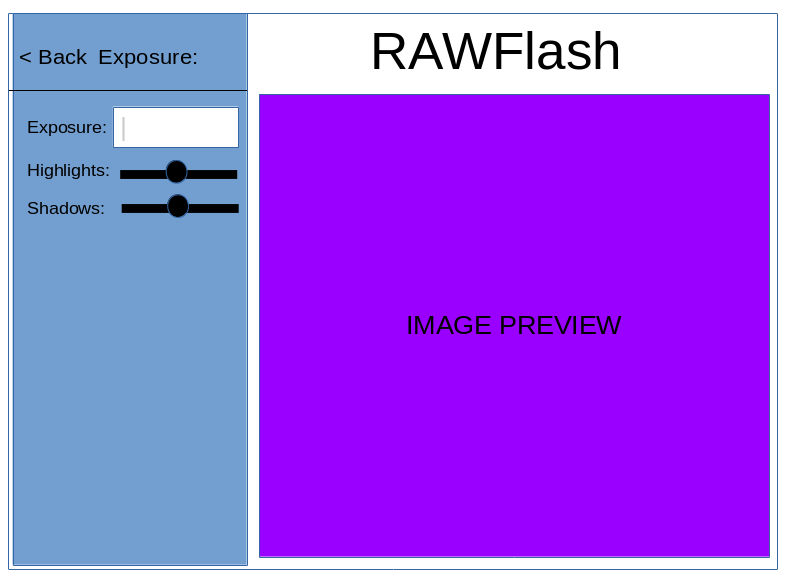
\includegraphics[width=0.5\textwidth]{uxdesign1}
  % \end{figure}

\subsection{Implementation Information}
Each individual module of the system requires different technologies in order to
produce an overall system.

\paragraph{Client-side Interface}
For this, HTML5, CSS3 and JavaScript (with jQuery to provide extra functionality)
are ideal, as HTML5 can be used to create the user interface, with CSS3 providing styling
and some basic animation to improve the UX. Using JavaScript with jQuery, it allows us
to keep track of the state of the editor, and transmit and receive information between client and
render server with help of some library. jQuery is useful for interfacing with the
DOM (the webpage itself, and it's components), allowing us to specify events, and functions
to run on particular events, along with template loading and various other functionalities.

As this is mostly static content, only a few web services needed for image selection/
maintaining user uploaded RAW files, a web server like Apache/NGINX can be used to serve
these static files, using server side scripting only to determine whether a user is authenticated,
and if so forwarding headers can be used to serve the static file without needing to serve static files
through the scripting language itself, which is much slower
\textbf{TODO: find source for static content and forwarding headers and performance.}

NGINX is what I'd recommend in this situation because unlike Apache, NGINX isn't
configured out of the box for dynamic content, but Apache is configured to use PHP
out of the box.

\paragraph{User account based RAW file management}
In order to select and upload images, a method of specifying users, and their uploaded
images needs to be created. This will require a database, to store the user information (username,
password), pointers to the images (image URL, and user associated with each image), along with some
server side scripts to manage authentication, dealing with file uploads, and maintaining collections
of images (listing all images associated with a user).

While any web framework would work with this, I've chosen to use the Python programming
language with the Django web framework, as database queries can be made using the built-in
Object Relational Mapper (ORM), that automatically writes SQL queries for the specified
database backend (e.g. MySQL, PostgreSQL), based on defining models as Python classes (inheriting
the django models.Model class).

Furthermore, Django contains built-in authentication, and built in methods to create users,
login, and managing sessions. These two features simplify the creation of the server side scripts
for user account based RAW file management.

For the interface, rather than sticking to server side generated pages, serving a JavaScript based
interface for this means the files can all be stored on the static file server used for the editor,
and therefore AJAX requests can be made to the server to get the information needed, and load them
onto the page. This avoids having to generate an entire page just for a few pieces of information. This
JavaScript code shall make a request to get a list of the images (encoded as JSON, along with their associated
urls). When a user clicks on the URL, the image picker loads up the editor, passing the URL to the image to edit (through
GET variables). This way, there is less reliance on the entire server side framework.

In order to ensure all of this works, a database is needed. Django officially supports three databases:
PostgreSQL, MySQL, Oracle and SQLite. SQLite is file based, and while it's ok for single user apps, for
multiple users it won't scale well. \textbf{TODO: reference for not using SQLite in production}.

MySQL is far better for applications, implementing most (but not all) of the SQL functionality. However,
it doesn't perform as well with concurrent users on write operations (e.g. writing new images into the database),
or writing the associated image settings to the database. Furthermore, features are missing like full text search.

 PostgreSQL is the most advanced, being fully standards compliant, and it has concurrency features built in to avoid using read locks.
 It's extensible, and allows for features like full text search. However, it can potentially be slower for primarily read based operations
 compared to MySQL, and as setup complexity for Postgres is far higher, it might not be the best tool for our project.

 Therefore, for this part of the system, Django shall be used alongside MySQL.
\paragraph{Render Server}
While lower level programming languages might be useful for image processing,
the requirement of linking this with web technologies means that a language such as C
or C++ is not as ideal.

Java is a better choice, as there are libraries available to provide web services (REST),
along with Web Socket implementations, along with Socket IO. Furthermore, Java contains
some libraries within the language that allow for image manipulation, most notably
BufferedImage related features such as ConvolveOp, image resizing, and various other standard
features build in. This is useful, as rather than starting completely from scratch, the custom
image processing routines can build on the built in Java implementations, and create more advanced
algorithms using them.

While Java doesn't support loading TIFF into BufferedReader using ImageIO directly,
an extension exists online, in the form of TwelveMonkeys. No RAW image loading library
exists within Java, but an executable such as dcraw or rawspeed can be used to generate a file
that can be read within Java, while retaining the quality (e.g. uncompressed TIFF). This can be done
using ProcessBuilder, and ideally writing a library to do this.
% of course, this library became jdcraw.

As this system will likely use a large amount of external dependencies, a dependency management tool
like Apache Maven should be used, to both manage dependencies from an external source (e.g. GitHub, Maven
Repositories), and also to build the system.
\textbf{TODO: reference libraries here.}

\begin{figure}[h]
    \centering
    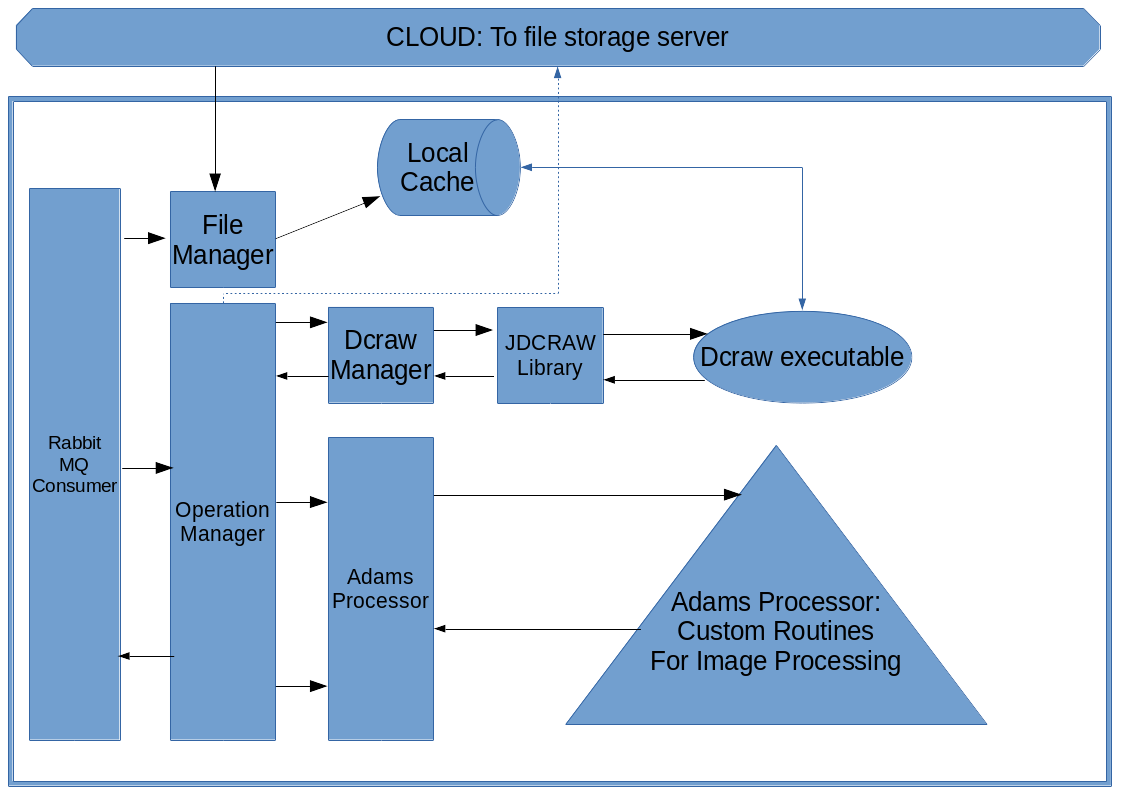
\includegraphics[width=0.25\textwidth]{renderserverdiagram}
    \caption{A diagram showing the structure of the render server components}
    \label{RenderServerDiagram}
\end{figure}
\begin{table}
  \centering
  \begin{tabular}{| c | p{12cm} | }
  \hline
  Number & Description\\
  1 & JSON string passed from server to file manager, to download/ensure the file is in the local cache.
  2 & If the file doesn't exist in cache (test using random number generator seed) download it from the file storage server.
  3 & Write the file to local cache if downloaded, using an aliased filename. Update the URL to this filename in the JSON string.
  4 & Pass the updated JSON string to the operation manager.
  5 & Pass the JSON String to the component dealing with rendering of RAW using DCRAW.
  6 & Parse JSON string, find the properties to modify within DCRAW and use the JDCRAW library to set up the executable.
  7 & Execute the instructions set up wtih the dcraw executable.
  8 & File will be read from the local cache, and processed by the executable.
  9 & The output of dcraw will be written back to the local cache, as a TIFF file (for compatibility with Java/Adams processor)
  10 & Pass the new rendered URL (the url of the tiff file) back up to JDCRAW library
  11 & Pass the URL up to the dcraw manager, and update the JSON string accordingly for the next processor in the pipeline.
  12 & Ensure the changes to the JSON string are reflected in the operation manager.
  13 & Pass the updated JSON string to the Adams Processor
  14 & Based on the operations defined in the JSON string, read the TIFF file (generated by DCRAW), and call the appropriate custom subroutines
  to process the image. These routines are written in Java, and are the custom written methods to create the advanced functionality.
  15 & Write the output of adams to a file, and pass the URL back up to the adams processor
  16 & Pass the JSON string up to the operation manager.
  17 & If an export grade image is needed, save the export file to the file storage server, and update the JSON string.
  18 & Export the appropriate information, including a base64 encoded preview of the image, and export URL if needed.

  \end{tabular}
  \caption{Render Server Steps Description}
  \label{RenderServerDiagramTable}
\end{table}

Overall, the render server system will be made up of several different components, each
confined to their
\paragraph{Account Management Server}
As this system needs to be used by multiple people, we need to have some record of users,
and their associated images.

Rather than rendering each page dynamically, we can instead use JavaScript to make AJAX requests,
fetching the data needed, and this way, we don't need to render whole HTML web pages. In terms of
backend technology, it doesn't matter too much what is used, as it won't be used too much, but
in my case I'll be using Node.JS with an Express server, simply because it's easy to deploy and
install dependencies ("npm install" can be run to install dependencies in one command), and it can
also connect to a database to provide services such as login, and records of individual files.

\paragraph{File Storage Server}
As the user is required to upload files, and the files that are exported need to be stored
somewhere (not on the render server local disk) to be accessed, it's important we have a
centralised store.

Ideally, this file storage server should be interchangable, allowing the user to change
where the files are stored (only requiring it to be accessable by using a URL).

There are a few options on the public cloud for use with this system, namely Amazon's S3,
and other storage services. However, as this prototype will initially be employed on a
private cloud, I shall use a service called OpenStack Swift, which allows the storage of files.
Furthermore, as this links in as a Django storage backend, and APIs already exist to tie Django in
with Swift, this makes the implementation easier. As this will be separate from the web services server,
and also seperate from the render server, any loss of either of these will cause the files to remain online,
and also allows for more user account management servers and more render servers to be placed online,
fetching and writing files to this file storage server.

\textbf{TODO Source: Why use OpenStack Swift}
\textbf{TODO: source: Django support for Open stack swift}

\paragraph{Distributed System Management}
As this system consists of several smaller systems, it's important that these are
managed. For each smaller component, a Docker container can be created, containing the
configuration between each one. From here, Docker Compose can then be used to manage
the entire system, bringing everything online, opening ports, and building everything
automatically.

This requires us to create a Dockerfile per system (one for the render server,
one for the client front-end). This Dockerfile specifies the image to build from,
along with instructions that need to be run, and files that should be shared, to make
that container work. Rather than customising an individual image, this customisation can be done
by building on existing images, saving time without needing to start again from scratch. \cite{DockerWhyItsUseful}

\textbf{TODO: some source of docker}
\subsection{Evaluation}
In order to measure the success of the system, a mixture of user based tests and system
based metrics will need to be taken.

As this is a software product, the underlying server will need to be constant to avoid
biased results. Therefore, for the tests, a computer shall be used as the server with the
following specs:

\begin{itemize}
  \item Processor: Intel i7-7700k at 4.2GHz
  \item Memory: 16GB DDR4-3000 RAM
  \item Storage: 1TB WD 7200RPM hard drive
  \item Operating System: Ubuntu 17.10
\end{itemize}

The amount of file storage here isn't as important, but as we are using a hard drive,
file caching might be slightly slower than if using an SSD.

The system will be deployed using Docker Compose, with the configuration scripts shown in the GitHub
repository.

\subsubsection{System-based Metrics}
Three different images per camera shall be used within the system to test compatibility
with other camera manufacturers. Canon, Nikon, Pentax and Lecia camera RAW formats shall be tested.
\textbf{SOURCE: top camera manufacturers, source of test images}.

In order to measure usability (along with the human based experiment), the system shall be used by
several different users, and for each, the time taken to submit a preview, and then get the preview displayed
on the screen shall be tested, as this figure gives us an indicataion in the delay between modifying parameters
and having the updated image displayed on screen.

\subsubsection{User-based tests}
While metrics can give us an indication into the usability and usefulness of the system,
it's also important to test the system with users.

The first test shall be carried out with individual users. This first test shall consist of
the following simple steps:

\begin{enumerate}
  \item Log into a given user account
  \item Create a new album
  \item Upload a new image to that album
  \item Open the image for editing in the editor
  \item Set the exposure to a specified value
  \item Adjust colour settings
  \item Use the built-in automated features
  \item Export the fixed image as PNG for download
\end{enumerate}

The users selected for this shall be mixed between experienced photographers (i.e. those
who are familar with using current RAW editing software such as Lightroom and Darktable), and
people who haven't used any RAW editing software before. The time taken for the users to carry
out the instructions shall be measured, along with their comments on the ease of use of the system through a survey.
The use of the time metric allows us to see how easy the system is to become familar with and to use, while the survey
allow us to compare the user's experience and how they found the software to use.

A sample of 10 people shall be used for the live demo, which while it isn't a very large sample size,
any sample size larger than this would make the tests difficult to carry out due to the requirement of external
application hosting.

\section{References}

% The list of cited references should appear at the end of the report, ordered alphabetically by the surnames of the first authors.  The default style for references cited in the main text is the  Harvard (author, date) format.  When citing a section in a book, please give the relevant page numbers, as in \cite[p293]{budgen}.  When citing, where there are either one or two authors, use the names, but if there are more than two, give the first one and use ``et al.'' as in  , except where this would be ambiguous, in which case use all author names.
%
% You need to give all authors' names in each reference.  Do not use ``et al.'' unless there are more than five authors.  Papers that have not been published should be cited as ``unpublished'' \cite{euther}.  Papers that have been submitted or accepted for publication should be cited as ``submitted for publication'' as in \cite{futher} .  You can also cite using just the year when the author's name appears in the text, as in ``but according to Futher \citeyear{futher}, we \dots''.  Where an authors has more than one publication in a year, add `a', `b' etc. after the year.

\bibliography{report}


\end{document}
